\section{Verification and reproducibility record}
\label{app:verification}

All inputs, scripts and reduced data are held in the repository
\texttt{github.com/contactrameezraja/}\allowbreak\texttt{quasicrystal-mace}, referred to throughout this appendix.

\subsection{Computational environment}
Production ran under the pinned module chain
PIP-PyTorch/2.4.0-foss-2023b-CUDA-12.4.0 with Python 3.11.5; the packages
carrying physics are mace, e3nn, phonopy and ase. Avon jobs ran on Quadro
RTX 6000 cards of 24~GB, of which approximately 22~GB is usable by the
runtime, and the largest run used a 47.7~GB L40 node on Blythe. The cached
potential checkpoints deserialise only under one version of the
equivariant-operations library, which the SevenNet requirements displace,
so one auxiliary environment was built solely for the SevenNet relaxations
and the primary environment is pinned rather than resolved afresh.

\subsection{Verification record}
The structure gate was tested by corruption, \texttt{verify\_parsers.py}
confirming that a deliberately corrupted fixture is refused at entry. The
spectral reduction guards against a trajectory whose atom count differs
from the supplied structure, terminating before any transform is
evaluated. The Wiener--Khinchin evaluation of the autocorrelation in
\texttt{reduce\_vdos.py} was checked against an explicit double loop over
time origins on a short trajectory during development, the two agreeing
to rounding; the loop is described in the script's docstring but is not
retained as a committed test. The displacement diagnostics were verified
on synthetic references with known answers, \texttt{msd\_gr.py --self-test}
generating one vibrating and one diffusing trajectory and recovering the
plateau and the $6Dt$ rise respectively.

The onset identification of Definition~\ref{def:floor} is by inspection
because no single threshold rule serves all the boxes. A rule declaring
the onset at the first energy above a reference $E_{\mathrm{ref}}$ at
which $g(E)$ exceeds a factor $F$ times $g(E_{\mathrm{ref}})$ was scanned
over $E_{\mathrm{ref}}$ from 0.3 to 1.0~meV and $F$ from 10 to 200. Over
the six calibration spectra the best single rule
($E_{\mathrm{ref}}=0.95$~meV, $F=50$) errs by 9~per cent on the smallest
box; required to serve the seventh spectrum as well, whose onset lies
below every usable reference energy, the best rule errs by 30~per cent.
The inspected onsets are justified by their outcome, the seven values
obeying the single relation of Section~4.5 whose prefactor an independent
route reproduces.

\subsection{Data and seeds}
Raw trajectories of approximately 24~GB are archived with the
force-constant files under a sha256 manifest; the force constants
regenerate from the repository inputs in sixteen to thirty-one minutes.
Seeds are recorded for every randomised step and production run except
the earliest $4\times4\times4$ box, as Section~3.5 notes, and the seeded
draw of the retargeted structure is archived as
\texttt{xbox\_wcomp.vasp}. The Monte Carlo searches are archived as
per-stage traces (\texttt{mq\_*\_trace.npy}) with their run logs; the
fixed-site validation is archived as its run log.

\subsection{Code listings}
\label{app:code}

The two routines on which the principal quantitative claims rest are
reproduced here verbatim from commit \texttt{b49a448} (23 August 2026) of the
repository named in Section~A.1. Every other script is mapped to its equations
in Table~\ref{tab:codemap} and is available at the same commit; these two are
listed because the spectra of Section~3.6 rest on the first and the factor-35
localisation contrast of Section~4.6.2 rests on the second.


\paragraph{Velocity autocorrelation and its cosine transform, Eqs.~(\ref{eq:vacf}) and~(\ref{eq:dos}).}
From \texttt{reduce\_vdos.py}. The autocorrelation is evaluated by the
Wiener--Khinchin relation with zero-padding to at least twice the sample
length, so that the linear rather than circular autocorrelation is obtained;
the density of states is the real part of the transform of the mirrored,
half-Hann-windowed correlation function, as Section~3.6 specifies. The
verification of this routine against an explicit double loop is recorded in Section~A.2.

\begin{lstlisting}
def vacf_fft(vel, masses, batch=64):
    """Mass-weighted VACF via Wiener-Khinchin, averaged over atoms and time
    origins. vel is (n_samples, n_atoms, 3). Atoms are processed in batches to
    keep the padded complex arrays a sensible size."""
    n_samples, n_atoms, _ = vel.shape
    n_fft = 1 << (2 * n_samples - 1).bit_length()      # >= 2N, power of two

    acc = np.zeros(n_samples)
    for start in range(0, n_atoms, batch):
        stop = min(start + batch, n_atoms)
        v = vel[:, start:stop, :].astype(np.float64)   # (n_samples, b, 3)
        f = np.fft.rfft(v, n=n_fft, axis=0)
        power = (f * np.conj(f)).real                  # |FFT|^2
        acf = np.fft.irfft(power, n=n_fft, axis=0)[:n_samples]
        acf = acf.sum(axis=2)                          # sum x,y,z -> (n_samples, b)
        # divide by the number of overlapping origins at each lag
        acf /= np.arange(n_samples, 0, -1)[:, None]
        acc += (acf * masses[start:stop][None, :]).sum(axis=1)

    acc /= acc[0]
    return acc


def vacf_to_vdos(vacf, dt):
    w = np.hanning(2 * len(vacf))[len(vacf):]          # half-Hann, decays at the tail
    vw = vacf * w
    full = np.concatenate([vw, vw[-1:0:-1]])           # mirror -> even function
    spec = np.maximum(np.real(np.fft.rfft(full)), 0)
    f = np.fft.rfftfreq(len(full), d=dt) / 1e12 * THZ_TO_MEV
    return f, spec
\end{lstlisting}

\paragraph{Participation ratio, Eqs.~(\ref{eq:siteweight}) and~(\ref{eq:partratio}).}
From \texttt{phonon\_run.py}. The site weight is the squared modulus of the
mass-weighted eigenvector summed over the three Cartesian components, and the
participation ratio follows the definition of Ref.~[1] so that the comparison
of Section~4.6.2 is on identical terms. The guard against a primitive-cell
mismatch is the check that catches the automatic primitive-cell reduction
described in Section~3.4.

\begin{lstlisting}
def participation_ratios(eigvecs, n_atoms):
    """eigvecs: (3N, n_modes) complex, columns are mass-weighted orthonormal
    eigenvectors as phonopy returns them. Returns P for each mode."""
    n_from_vec = eigvecs.shape[0] // 3
    if n_from_vec != n_atoms:
        raise SystemExit(f'eigenvector length implies {n_from_vec} atoms but '
                         f'{n_atoms} were passed: primitive-cell mismatch')
    e = eigvecs.reshape(n_atoms, 3, eigvecs.shape[-1])
    p_site = (np.abs(e) ** 2).sum(axis=1)            # (n_atoms, n_modes)
    p_site = p_site / p_site.sum(axis=0, keepdims=True)
    return 1.0 / (n_atoms * (p_site ** 2).sum(axis=0))
\end{lstlisting}

\paragraph{Structure files.}
The deposited and relaxed structures are archived in the repository as
\texttt{Al9Co2Ni2-coords.txt} (X-phase, legacy coordinate format carrying the
refined ordering of Ref.~[14]), \texttt{W-AlCoNi-265.vasp} and
\texttt{W-AlCoNi-265-relaxed.vasp} (W-phase, deposited and relaxed),
\texttt{al13co4.vasp} (periodic control) and \texttt{xbox\_wcomp.vasp}
(retargeted box). The generation searches of Section~4.11 are archived as
their best structures (\texttt{mq\_*\_best.vasp}) alongside the per-stage
traces (\texttt{mq\_*\_trace.npy}).
\clearpage
\label{app:figs}

\begin{table}[H]
\centering
\caption[Repository code mapped to the equations implemented]{Repository
scripts mapped to the equations of Chapter~3 and the outputs of Chapter~4.}
\label{tab:codemap}
\small
\begin{tabular}{p{0.28\textwidth}p{0.38\textwidth}p{0.26\textwidth}}
\toprule
Script & Implements & Output \\
\midrule
\texttt{md\_run.py} & relaxation to Eq.~(\ref{eq:fmax}); the dynamics
  protocol of \S3.5 & trajectories, drift logs \\
\texttt{reduce\_vdos.py} & Eqs.~(\ref{eq:vacf}), (\ref{eq:dos}); segment
  and length statistics of \S3.9; the trajectory atom-count guard &
  $g(E)$, element projections \\
\texttt{gvdos.py} & neutron weighting, Eq.~(\ref{eq:neutron}) & $G(E)$ \\
\texttt{phonon\_run.py} & Eqs.~(\ref{eq:dynmat})--(\ref{eq:partratio});
  the band paths and gap extraction of \S3.4 & mode sets, $P(s)$,
  boundary gap centres \\
\texttt{msd\_gr.py} & Eqs.~(\ref{eq:msd}), (\ref{eq:lindemann}); pair
  distribution functions & Table~\ref{tab:msd} \\
\texttt{melt\_quench.py} & Eq.~(\ref{eq:metropolis}); the melt-quench,
  replica-exchange and fixed-site modes of \S3.10 & search traces, best
  structures \\
\texttt{retarget\_composition.py} & the seeded site reassignment of
  \S3.2.2 & the retargeted structure \\
\texttt{verify\_parsers.py} & first-entry verification of \S3.2,
  including rejection of a corrupted fixture & gate records \\
\texttt{fig\_structures.py}, \texttt{make\_fig9.py}; notebooks
  \texttt{O2\_Phonopy}, \texttt{O2\_MD}, \texttt{O3\_figures} & figure
  generation from archived reduction outputs & Figures~4, 5, 7 to 9, 11,
  12, 15 to 19 \\
\texttt{make\_fig\_floor.py} & the floor calibration of \S4.5 against
  the box lengths of the run logs & Figure~6 \\
\texttt{make\_fig\_pseudogap.py}, \texttt{make\_fig\_workflow.py} &
  the illustrative construction of \S2.1; the workflow diagram &
  Figures~2, 3 \\
\texttt{make\_fig\_sq.py}, \texttt{make\_fig\_gr.py} & the structure
  factor of the $6\times2\times1$ box at its allowed wavevectors; the
  archived $g(r)$ reductions replotted & Figures~13, 14 \\
\texttt{make\_fig\_stacking\_centres.py} & the stacking gap-centre
  ladder of \S4.6.3, from the archived record
  \texttt{stacking\_bandpath\_gaps.txt} & Figure~10 \\
\texttt{fig\_onset\_definition.py} & sensitivity of the onset to the
  Definition~\ref{def:floor} threshold factor, the prefactor refitted at
  factors 5, 10 and 20 across the six calibration boxes & prefactor
  sensitivity record \\
\bottomrule
\end{tabular}
\end{table}
\clearpage

\subsection{Supplementary figures}

Four diagnostic figures from the production record are collected here.
Each supports a number or a claim made in the body and is cited there
by section; none introduces a result not already reported. All were
generated from the archived reduction outputs by the notebooks and
scripts of Table~\ref{tab:codemap} at the commit named in Section~A.4.

\begin{figure}[!ht]
\centering
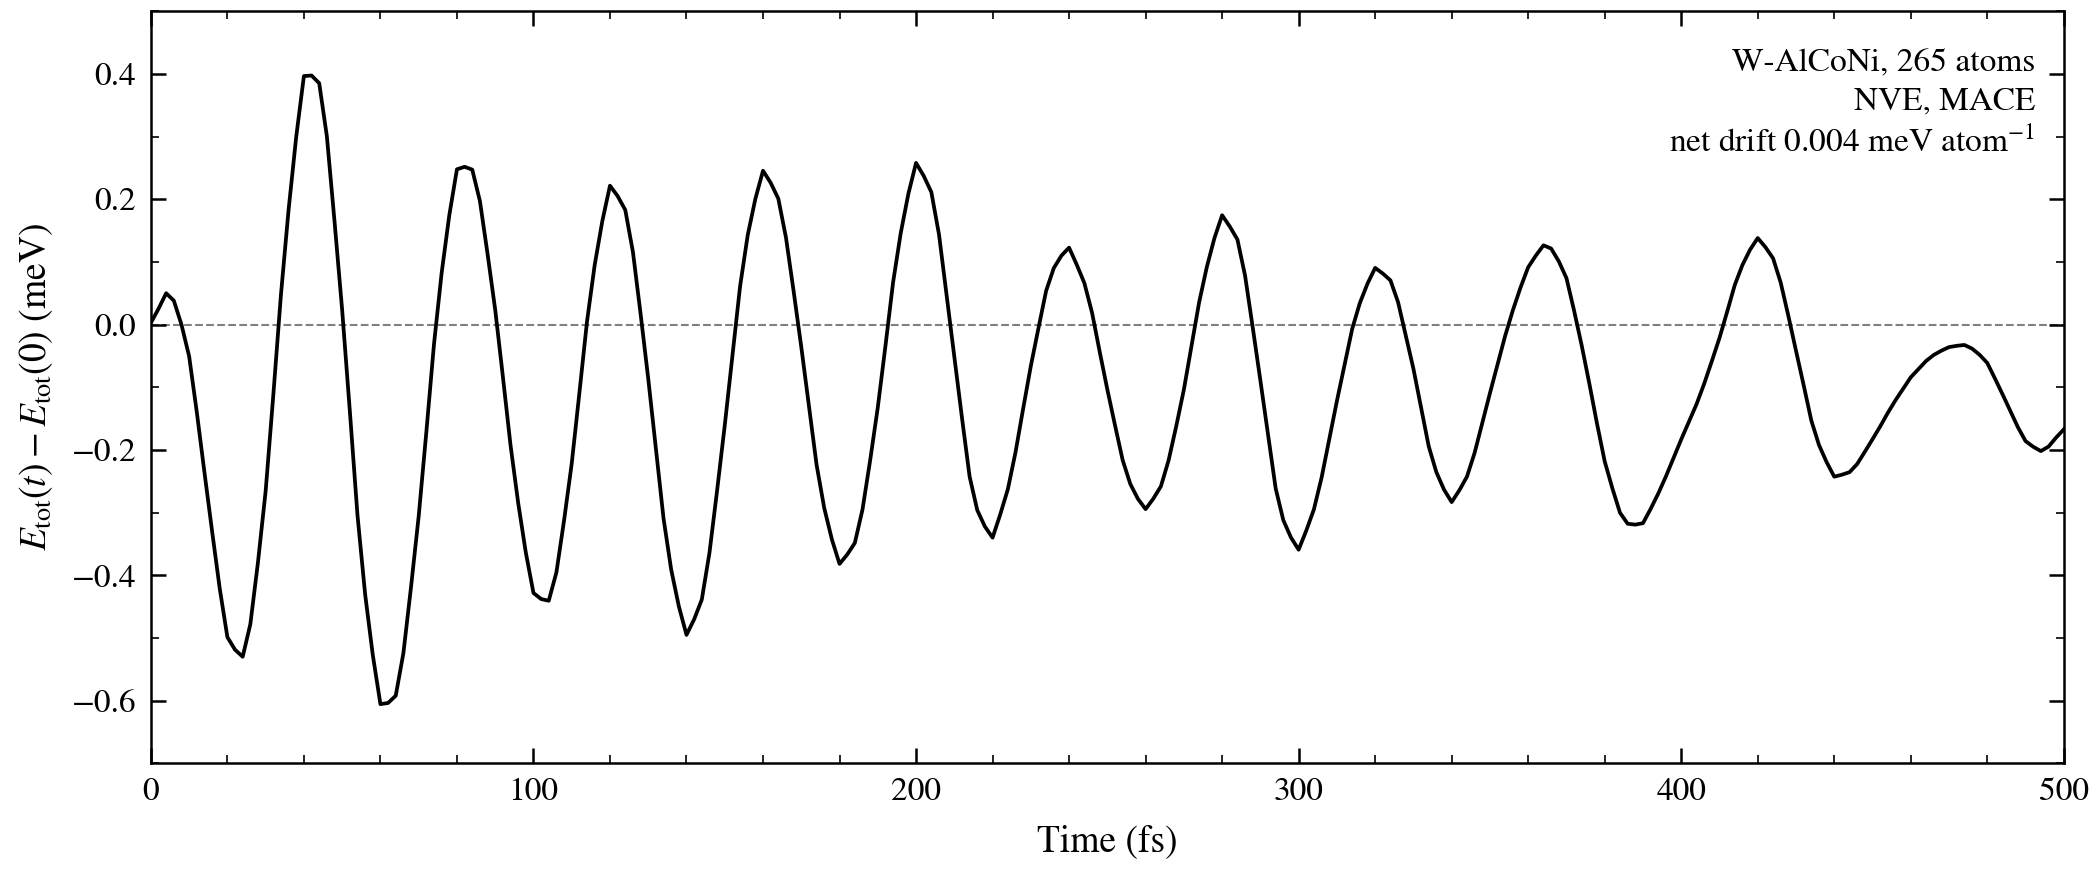
\includegraphics[width=0.9\textwidth]{nve_energy_conservation.png}
\caption[Integrator stability segment]{Total-energy excursion over the
0.5~ps microcanonical stability
segment for the 265-atom W-phase under MACE-MPA-0. The net drift of
0.004~meV per atom is the integrator reference against which every
production drift of Table~\ref{tab:runs} is compared (Section~4.2); the
oscillation is the reversible exchange between kinetic and potential
energy at the period of the dominant modes, not a drift.}
\label{fig:app_nve}
\end{figure}

\begin{figure}[!ht]
\centering
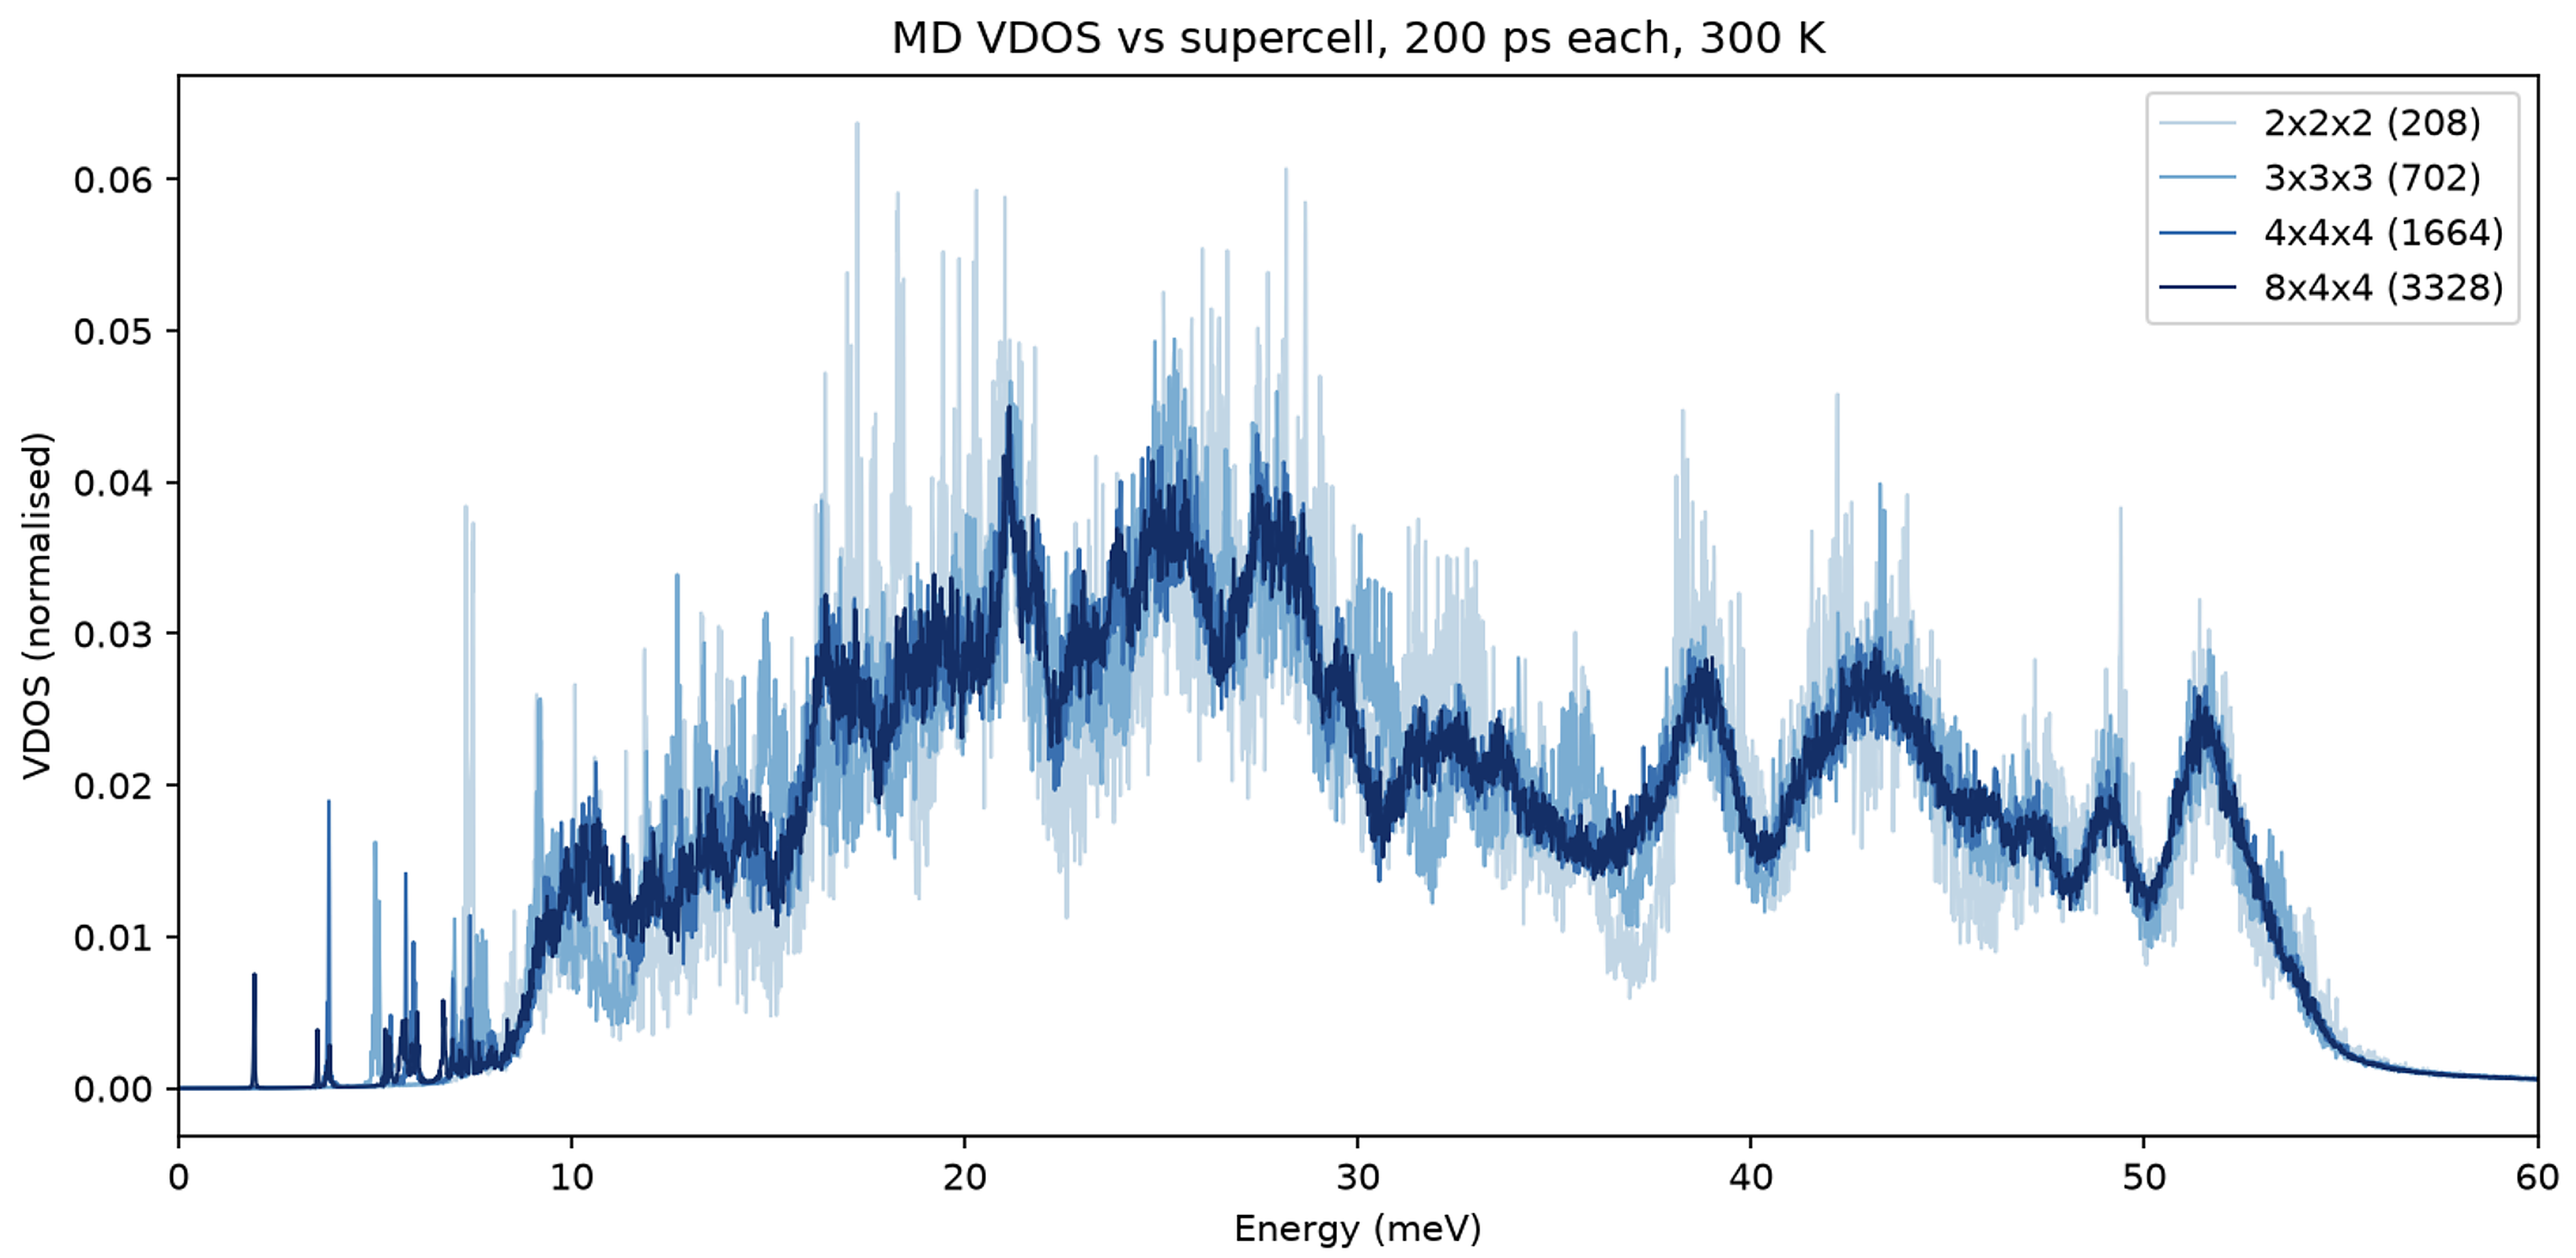
\includegraphics[width=0.9\textwidth]{md_vdos_supercell_sharpened.png}
\caption[Size convergence of the X-phase spectra]{Velocity-autocorrelation spectra of the four X-phase production boxes of Table~\ref{tab:runs}, 200~ps each at 300~K. The lowest sharp
feature moves to lower energy as the longest box dimension grows, from
6.24~meV at $2\times2\times2$ to 1.83~meV at $8\times4\times4$, while the
spectrum above 10~meV converges; these are the onsets tabulated in
Table~\ref{tab:floor} before the relation of Section~4.5 was fitted to
them.}
\label{fig:app_series}
\end{figure}

\begin{figure}[!ht]
\centering
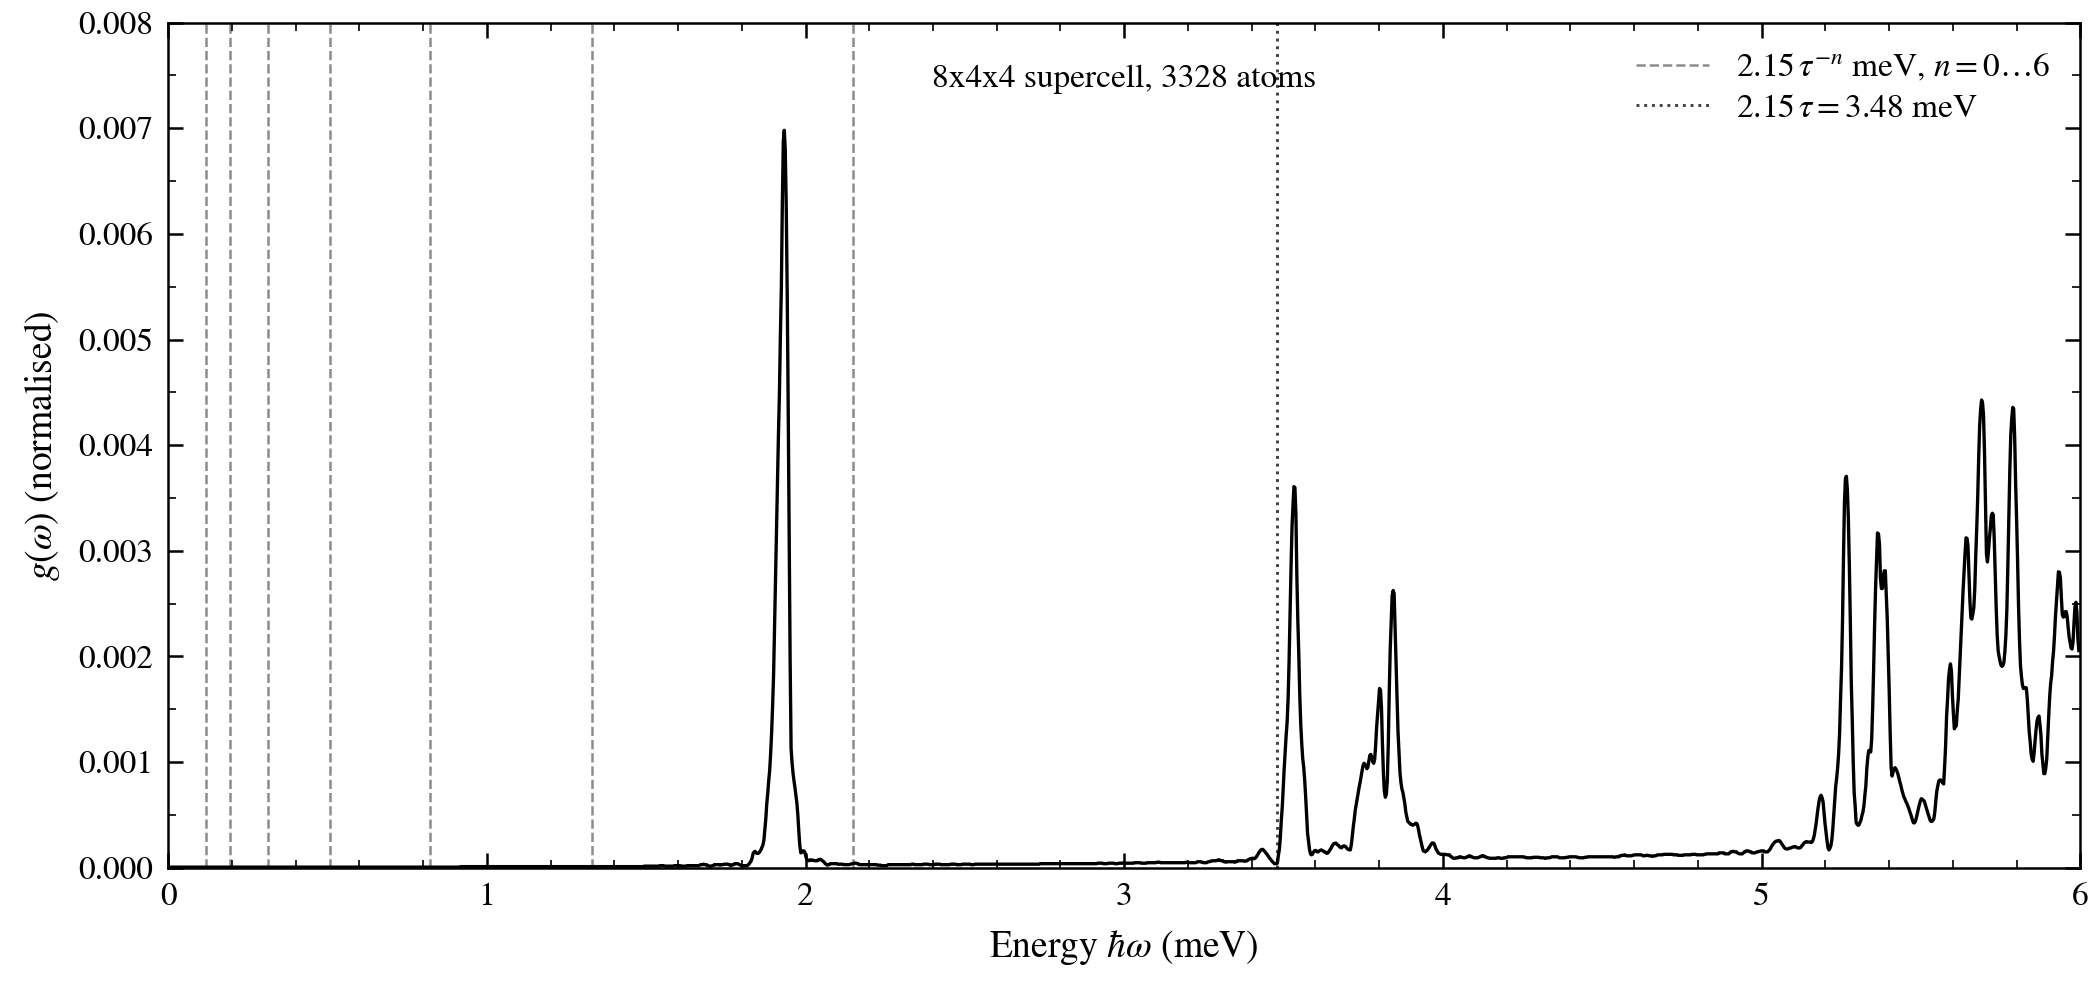
\includegraphics[width=0.9\textwidth]{vdos_lowE_8x4x4_ladder.png}
\caption[The $8\times4\times4$ spectrum against the measured ladder]{Low-energy
spectrum of the $8\times4\times4$ X-phase box (3328
atoms) against the measured ladder of Ref.~[2], each rung
$2.15\,\tau^{-n}$~meV drawn as a dashed line and $2.15\,\tau=3.48$~meV
dotted. The 2.15~meV rung lies in a region of near-baseline weight between
the dominant features at 1.93 and 3.54~meV, and nothing lies at 3.48~meV,
the observations of Section~4.5.1.}
\label{fig:app_ladder}
\end{figure}

\begin{figure}[t]
\centering
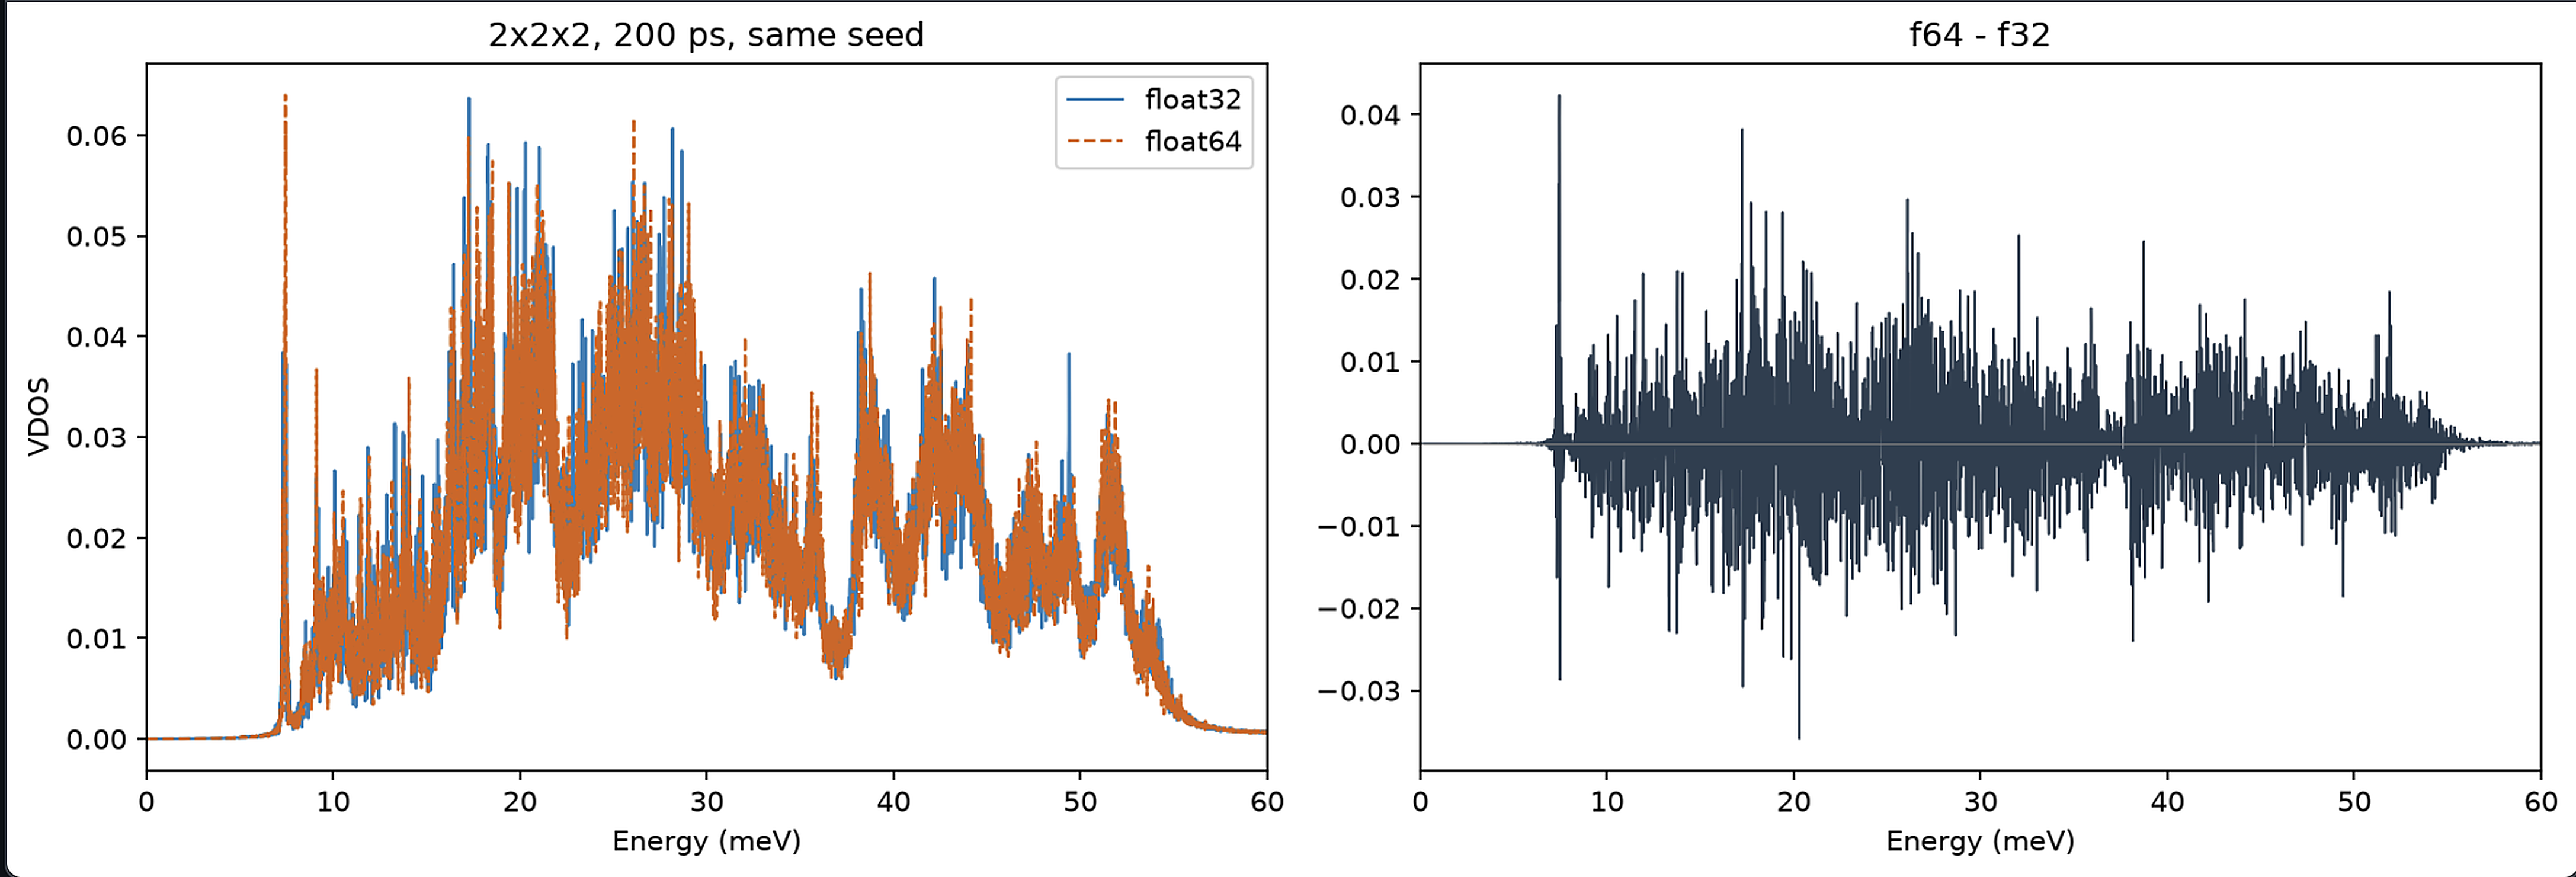
\includegraphics[width=\textwidth]{f32_vs_f64_vdos_sharpened.png}
\caption[The precision experiment]{The precision experiment of
Sections~3.9 and~4.10. Left, the
$2\times2\times2$ X-phase spectrum from single- and double-precision
runs of 200~ps from one seed; right, their difference. The difference is
symmetric about zero with no systematic offset, which is why the
22.65~per~cent spectral difference is treated as run-to-run scatter of two
decorrelated trajectories rather than as a precision effect.}
\label{fig:app_prec}
\end{figure}